\section{Introduction}
\label{introduction}

% state the learning objective 
The aim of this laboratory work regarding the topics studied in the first three weeks of the course was to analyse a circuit constituted of an independent voltage source, an independent voltage source, a voltage controlled dependent current source, a current controlled dependent voltage source and seven resistors, as shown in the Figure t1draw below.
. For this, a theorical analysis was made using both node and mesh methods, whose results will be discussed in section one. To validate these results, a simulation was conducted, as will apeear in section 2.


The forementioned analysis was divided into a theoretical one, presented in section .In order to be able to validate the results obtained, a simulation was also conducted, as shown in Section . The results were then compared , and the conclusions of the group summarized in Section 


\begin{figure}[h] \centering
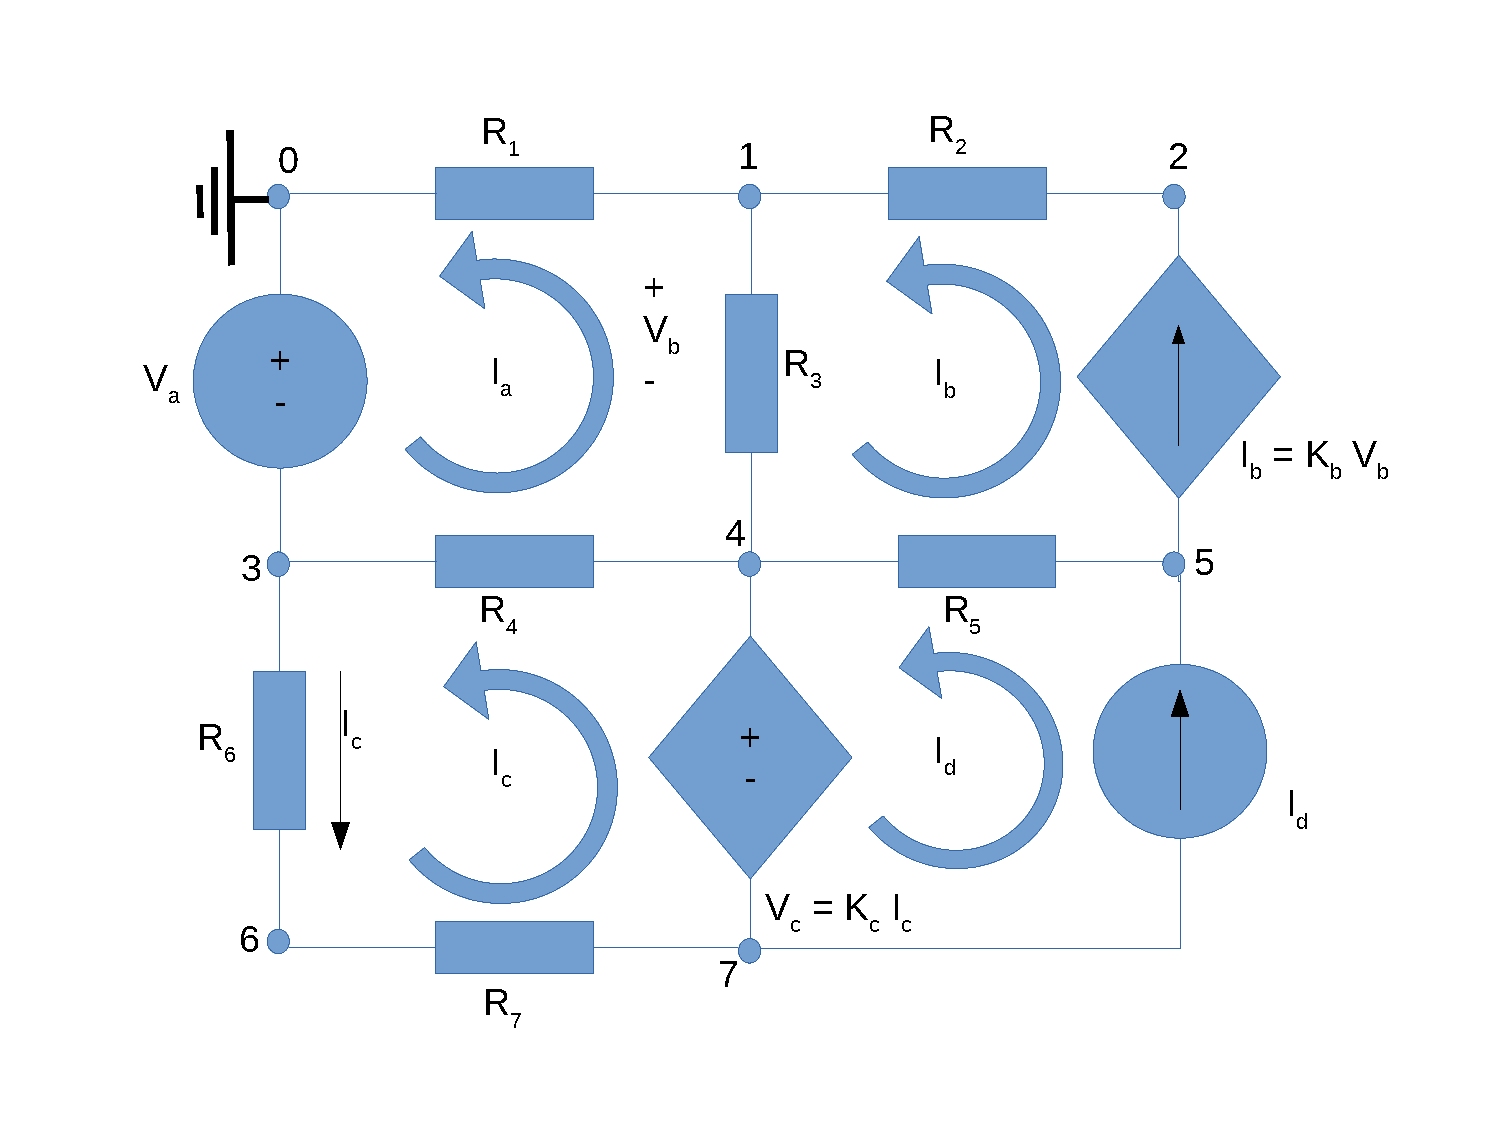
\includegraphics[width=0.7\linewidth]{t1draw.pdf}
\caption{Circuit analysed.}
\label{t1draw}
\end{figure}


